\documentclass[tikz,border=8pt]{standalone}
% Shared look for every TikZ diagram. Load with \input{../../tools/tikz-style.tex}
\usepackage[T1]{fontenc}
\usepackage{lmodern}
\renewcommand{\sfdefault}{lmr}  % diagrams use the same serif as the text
\usetikzlibrary{arrows.meta, positioning, shapes.geometric, calc, fit, backgrounds}
\definecolor{cblue}{HTML}{4C78A8}
\definecolor{corange}{HTML}{F58518}
\definecolor{cgreen}{HTML}{54A24B}
\definecolor{cred}{HTML}{E45756}
\definecolor{cpurple}{HTML}{B279A2}
\definecolor{cgrey}{HTML}{6B6B6B}
\tikzset{
  every picture/.style={font=\sffamily, line width=1.2pt},
  box/.style={draw=#1, fill=#1!12, rounded corners=4pt, align=center, inner sep=7pt, minimum height=1.1cm},
  box/.default=cgrey,
  arrow/.style={-{Stealth[length=3mm]}, draw=cgrey, line width=1.4pt},
  title/.style={font=\sffamily\bfseries\Large},
  note/.style={font=\sffamily\small, text=cgrey, align=center},
}
\AtBeginDocument{\hyphenpenalty=10000 \exhyphenpenalty=10000}

% Two robots on a smooth floor, motors off, both at 2 m now. A stood still (it was at 2 m a second ago); B rolls at
% 0.5 m/s (it was at 1.5 m). One second later A is at 2 m, B at 2.5 m: position alone does not predict the future.
\begin{document}
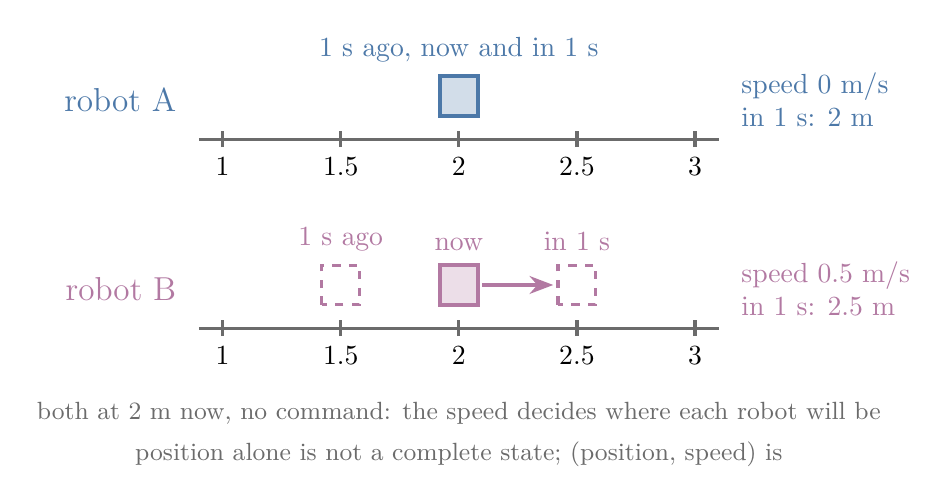
\begin{tikzpicture}[x=3cm, y=1cm, every node/.append style={font=\large}]
  \foreach \row in {0,-2.4} {
    \draw[cgrey, line width=1pt] (0.9,\row) -- (3.1,\row);
    \foreach \t in {1,1.5,2,2.5,3} { \draw[cgrey] (\t,\row-0.1) -- (\t,\row+0.1); \node[below, font=\normalsize] at (\t,\row-0.1) {\t}; }
  }
  % robot A: still
  \node[left, cblue] at (0.85,0.5) {robot A};
  \draw[cblue, fill=cblue!25, line width=1.5pt] (1.92,0.3) rectangle (2.08,0.8);
  \node[cblue, above, font=\normalsize] at (2,0.85) {1 s ago, now and in 1 s};
  \node[right, cblue, font=\normalsize, align=left] at (3.15,0.5) {speed 0 m/s\\in 1 s: 2 m};
  % robot B: rolling
  \begin{scope}[yshift=-2.4cm]
    \node[left, cpurple] at (0.85,0.5) {robot B};
    \draw[cpurple, dashed] (1.42,0.3) rectangle (1.58,0.8); \node[cpurple, above, font=\normalsize] at (1.5,0.85) {1 s ago};
    \draw[cpurple, fill=cpurple!25, line width=1.5pt] (1.92,0.3) rectangle (2.08,0.8); \node[cpurple, above, font=\normalsize] at (2,0.85) {now};
    \draw[cpurple, dashed] (2.42,0.3) rectangle (2.58,0.8); \node[cpurple, above, font=\normalsize] at (2.5,0.85) {in 1 s};
    \draw[-{Stealth[length=3mm]}, cpurple, line width=1.5pt] (2.1,0.55) -- (2.4,0.55);
    \node[right, cpurple, font=\normalsize, align=left] at (3.15,0.5) {speed 0.5 m/s\\in 1 s: 2.5 m};
  \end{scope}
  \node[note, anchor=north] at (2,-3.2) {both at 2 m now, no command: the speed decides where each robot will be};
  \node[note, anchor=north] at (2,-3.7) {position alone is not a complete state; (position, speed) is};
\end{tikzpicture}
\end{document}
